\documentclass[polish,polish,a4paper]{article}
\usepackage[polish]{babel}
\usepackage[T1]{fontenc}
\usepackage[utf8]{inputenc}
\usepackage{pslatex}
\usepackage{pgfplots}
\usepackage{circuitikz} 
\usepackage{setspace}
\usepackage{caption}
\usepackage{amssymb}
\usepackage{amsmath}
%\usetikzlibrary{circuits.ee.IEC}
\usepackage{anysize}
\usepackage{graphicx}
\usepackage{hyperref}
\usepackage{float}
\hypersetup{
	colorlinks=true,
	linkcolor=blue,
	filecolor=magenta,      
	urlcolor=cyan,
}

\marginsize{2.5cm}{2.5cm}{2cm}{2cm}

\newcommand{\PRzFieldDsc}[1]{\sffamily\bfseries\scriptsize #1}
\newcommand{\PRzFieldCnt}[1]{\textit{#1}}
\newcommand{\PRzHeading}[8]{
	%% #1 - nazwa laboratorium
	%% #2 - kierunek 
	%% #3 - specjalność 
	%% #4 - rok studiów 
	%% #5 - symbol grupy lab.
	%% #6 - temat 
	%% #7 - numer lab.
	%% #8 - skład grupy ćwiczeniowej
	
	\begin{center}
		\begin{tabular}{ p{0.32\textwidth} p{0.15\textwidth} p{0.15\textwidth} p{0.12\textwidth} p{0.12\textwidth} }
			
			&   &   &   &   \\
			\hline
			\multicolumn{5}{|c|}{}\\[-1ex]
			\multicolumn{5}{|c|}{{\LARGE #1}}\\
			\multicolumn{5}{|c|}{}\\[-1ex]
			
			\hline
			\multicolumn{1}{|l|}{\PRzFieldDsc{Kierunek}}	& \multicolumn{1}{|l|}{\PRzFieldDsc{Specjalność}}	& \multicolumn{1}{|l|}{\PRzFieldDsc{Rok studiów}}	& \multicolumn{2}{|l|}{\PRzFieldDsc{Symbol grupy lab.}} \\
			\multicolumn{1}{|c|}{\PRzFieldCnt{#2}}		& \multicolumn{1}{|c|}{\PRzFieldCnt{#3}}		& \multicolumn{1}{|c|}{\PRzFieldCnt{#4}}		& \multicolumn{2}{|c|}{\PRzFieldCnt{#5}} \\
			
			\hline
			\multicolumn{4}{|l|}{\PRzFieldDsc{Temat Laboratorium}}		& \multicolumn{1}{|l|}{\PRzFieldDsc{Numer lab.}} \\
			\multicolumn{4}{|c|}{\PRzFieldCnt{#6}}				& \multicolumn{1}{|c|}{\PRzFieldCnt{#7}} \\
			
			\hline
			\multicolumn{5}{|l|}{\PRzFieldDsc{Skład grupy ćwiczeniowej oraz numery indeksów}}\\
			\multicolumn{5}{|c|}{\PRzFieldCnt{#8}}\\
			
			\hline
			\multicolumn{3}{|l|}{\PRzFieldDsc{Uwagi}}	& \multicolumn{2}{|l|}{\PRzFieldDsc{Ocena}} \\
			\multicolumn{3}{|c|}{\PRzFieldCnt{\ }}		& \multicolumn{2}{|c|}{\PRzFieldCnt{\ }} \\
			
			\hline
		\end{tabular}
	\end{center}
}



\begin{document}


	\PRzHeading{Laboratorium Podstaw Elektroniki}{Informatyka}{--}{I}{I3}{Twierdzenie Thevenina}{2}{Piotr Więtczak(132339), Robert Ciemny(136693), Kamil Basiukajc(136681)}
	\begin{spacing}{2}
	\section{Cel zadania}
	Celem tego zadania jest dokonanie odpowiednich pomiarów w przedstawionym przez prowadzącego układzie,a następnie korzystając z twierdzenia Thevenina obliczyć wartości prądów $I_{1}, I_{2}, I_{3}$, oraz wykonać to samo przy pomocy obliczeń analityczne. Na koniec podać zastosowania twierdzenia Thevenina.
	
	\section{Budowa wskazanej konfiguracji przy pomocy środków dostępnych na stanowisku laboratoryjnym.}
	
	\begin{equation*}
	\begin{circuitikz}[american]
	\draw
	(0,0) to [european resistor,l= $R_{1}$, a = $220\Omega$] (0,3)
	to[short, -*]  (3,3)
	to[short, -*]  (6,3)
	to [european resistor, l=$R_{5}$, a=$220\Omega$] (9,3)
	to  [V, l=$5V$] (9,0)
	to [european resistor, a=$R_{4}$, l =$1k\Omega$] (6,0)
	to[short,*-*] (3,0)
	to (0,0)
	(3,0) to [european resistor, l=$R_{2}$, a = $1k\Omega$] (3,3)
	(6,0) to [european resistor, l=$R_{3}$, a = $2.2k\Omega$] (6,3);
	\end{circuitikz}
	\end{equation*}
	\captionof{figure}{Schemat badanego obwodu.}
	
	\begin{figure}[H]
		\centering
		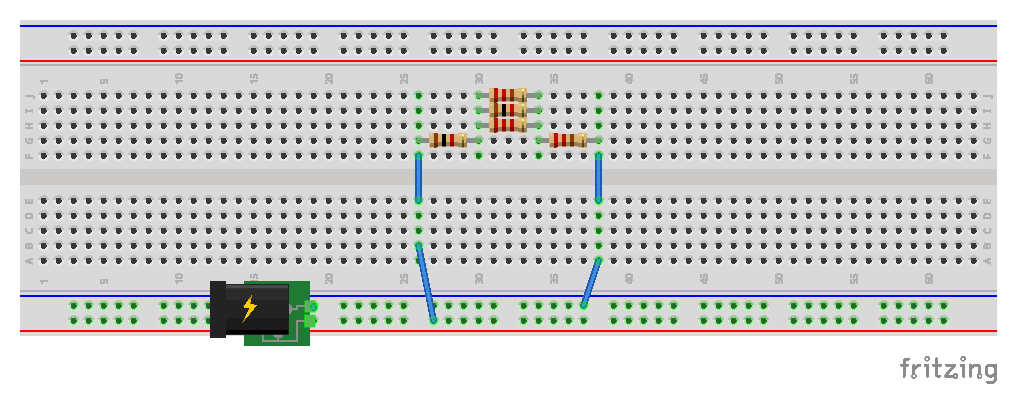
\includegraphics[scale=0.8]{startowy_bb.pdf}
		\captionof{figure}{Schemat badanego obwodu wykonany w programie Fritzing.}
	\end{figure}
	
	\section{Obliczenie wartości prądów $I_{1},I_{2},I_{3}$}
	\subsection{$I_{1}$}
	\subsubsection{Korzystając z twierdzenia Thevenina}
	Pomiar $U_{th}$ po wyeliminowaniu rezystora $R_{1}$ przy  użyciu multimetru skonfigurowanego do pomiaru napięcia. Multimetr wskazał wynik: $1.824V$.
	\begin{figure}[H]
		\centering
		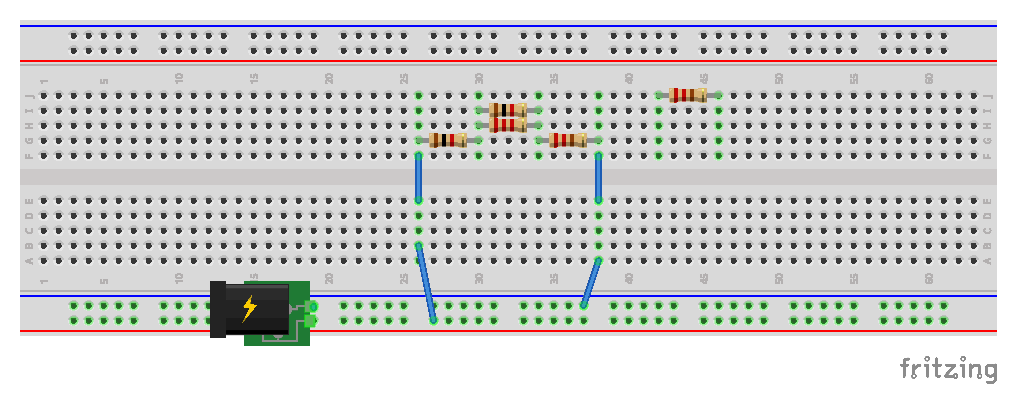
\includegraphics[scale=0.8]{R1_pomiar_napiecia_bb.pdf}
		\captionof{figure}{Schemat badanego obwodu przygotowanego do pomiaru napięcia.}
	\end{figure}

	Zastąpienie źródła napięcia i pomiar rezystancji zastępczej $R_{th}$ przy użyciu multimetru skonfigurowanego do pomiaru rezystancji. Multimetr wskazał wynik: $ 434,202\Omega $.
	\begin{figure}[H]
		\centering
		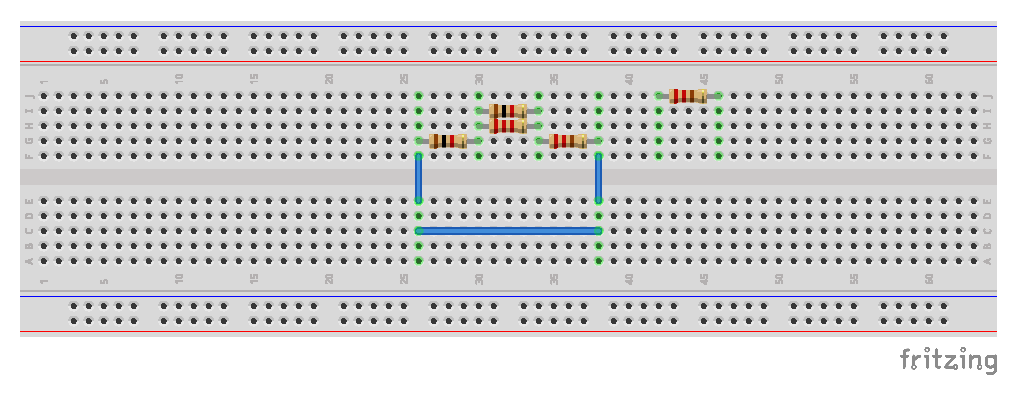
\includegraphics[scale=0.8]{R1_pomiar_oporu_bb.pdf}
		\captionof{figure}{Schemat badanego obwodu przygotowanego do pomiaru rezystancji zastępczej.}
	\end{figure}
	Wyznaczenie prądu $I_{1}$, z wartości otrzymanych podczas pomiarów, przy pomocy wzoru: $I_{x}= \dfrac{U_{thx}}{R_{thx} + R_{x}}$.
	\begin{gather*}
		I_{1}=\dfrac{1.824V}{434.202\Omega + 220\Omega } = 2.788mA
	\end{gather*}
	\subsubsection{Przy pomocy obliczeń analitycznych}
	Obliczenie $U_{ht}$ przy wyeliminowanym oporniku $ R_{1} $.
	\begin{gather*}
	U_{th}= \dfrac{V_{1}}{R_{4}+R_{5}+R_{23}} \cdot R_{23}\\
	R_{23} = \dfrac{R_{2} \cdot R_{3}}{R_{2} + R_{3}}\\
	R_{23} = \dfrac{2200\Omega \cdot 1000\Omega}{2200\Omega + 1000\Omega} = 687.5\Omega\\
	U_{th} = \dfrac{5V}{1000\Omega + 220\Omega + 689.5\Omega } \cot 687.5\Omega\\
	U_{th} = 1.802V
	\end{gather*}
	Obliczenie $R_{ht}$ przy wyeliminowanym oporniku $ R_{1} $.
	\begin{gather*}
		R_{23} = \dfrac{1}{\dfrac{1}{R_{2}} + \dfrac{1}{R_{3}}}\\
		R_{45} = R_{4} + R_{5}\\
		R_{th} = \dfrac{1}{\dfrac{1}{R_{23}} + \dfrac{1}{R_{45}}} = \dfrac{1}{\dfrac{1}{\dfrac{1}{\dfrac{1}{R_{2}} + \dfrac{1}{R_{3}}}} + \dfrac{1}{R_{4} + R_{5}}}\\
			R_{th} = \dfrac{1}{\dfrac{1}{\dfrac{1}{\dfrac{1}{2200\Omega} + \dfrac{1}{2200\Omega}}} + \dfrac{1}{1000\Omega + 220\Omega}} \approx 439,712\Omega
	\end{gather*}
	Wyznaczenie prądu $I_{1}$, z wartości otrzymanych podczas obliczeń, przy pomocy wzoru: $I_{x}= \dfrac{U_{thx}}{R_{thx} + R_{x}}$.
	\begin{gather*}
	I_{1}=\dfrac{1.802V}{439,712\Omega + 220\Omega } = 2.732mA
	\end{gather*}
	\subsection{$I_{2}$}
		\subsubsection{Korzystając z twierdzenia Thevenina}
			Pomiar $U_{th}$ po wyeliminowaniu rezystora $R_{2}$ przy  użyciu multimetru skonfigurowanego do pomiaru napięcia. Multimetr wskazał wynik: $0.749V$.
		\begin{figure}[H]
			\centering
			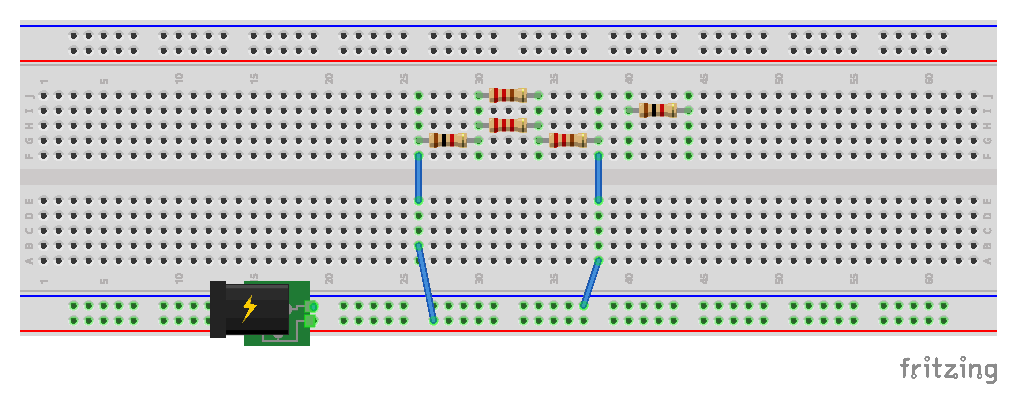
\includegraphics[scale=0.8]{R2_pomiar_napiecia_bb.pdf}
			\captionof{figure}{Schemat badanego obwodu przygotowanego do pomiaru napięcia.}
		\end{figure}
		
		Zastąpienie źródła napięcia i pomiar rezystancji zastępczej $R_{th}$ przy użyciu multimetru skonfigurowanego do pomiaru rezystancji. Multimetr wskazał wynik: $ 168.841\Omega $.
		\begin{figure}[H]
			\centering
			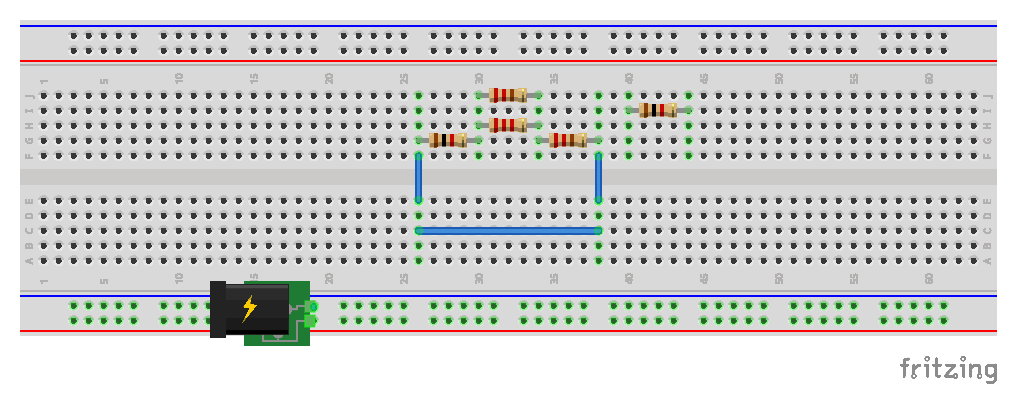
\includegraphics[scale=0.8]{R2_pomiar_oporu_bb.pdf}
			\captionof{figure}{Schemat badanego obwodu przygotowanego do pomiaru rezystancji zastępczej.}
		\end{figure}
		Wyznaczenie prądu $I_{2}$, z wartości otrzymanych podczas pomiarów, przy pomocy wzoru: $I_{x}= \dfrac{U_{thx}}{R_{thx} + R_{x}}$.
		\begin{gather*}
		I_{2}=\dfrac{0.749V}{171,831\Omega + 1000\Omega } = 0.641mA
		\end{gather*}
	\subsubsection{Przy pomocy obliczeń analitycznych}
	Obliczenie $U_{ht}$ przy wyeliminowanym oporniku $ R_{2} $.
		\begin{gather*}
	U_{th}= \dfrac{V_{1}}{R_{4}+R_{5}+R_{13}} \cdot R_{13}\\
	R_{13} = \dfrac{R_{1} \cdot R_{3}}{R_{1} + R_{3}}\\
	R_{13} = \dfrac{220\Omega \cdot 2200\Omega}{2420\Omega} = 200\Omega\\
	U_{th} = \dfrac{5V}{1000\Omega + 220\Omega + 200\Omega } \cot 200\Omega\\
	U_{th} = 0.704V
	\end{gather*}
	Obliczenie $R_{ht}$ przy wyeliminowanym oporniku $ R_{2} $.
	\begin{gather*}
	R_{13} = \dfrac{1}{\dfrac{1}{R_{1}} + \dfrac{1}{R_{3}}}\\
	R_{45} = R_{4} + R_{5}\\
	R_{th} = \dfrac{1}{\dfrac{1}{R_{13}} + \dfrac{1}{R_{45}}} = \dfrac{1}{\dfrac{1}{\dfrac{1}{\dfrac{1}{R_{1}} + \dfrac{1}{R_{3}}}} + \dfrac{1}{R_{4} + R_{5}}}\\
	R_{th} = \dfrac{1}{\dfrac{1}{\dfrac{1}{\dfrac{1}{220\Omega} + \dfrac{1}{2200\Omega}}} + \dfrac{1}{1000\Omega + 220\Omega}} \approx 171,831\Omega
	\end{gather*}
		Wyznaczenie prądu $I_{2}$, z wartości otrzymanych podczas obliczeń, przy pomocy wzoru: $I_{x}= \dfrac{U_{thx}}{R_{thx} + R_{x}}$.
	\begin{gather*}
	I_{2}=\dfrac{0.704V}{168.841 + 1000\Omega } = 0.602mA
	\end{gather*}
	\subsection{$I_{3}$}
		\subsubsection{Korzystając z twierdzenia Thevenina}
					Pomiar $U_{th}$ po wyeliminowaniu rezystora $R_{3}$ przy  użyciu multimetru skonfigurowanego do pomiaru napięcia. Multimetr wskazał wynik: $0.658V$.
		\begin{figure}[H]
			\centering
			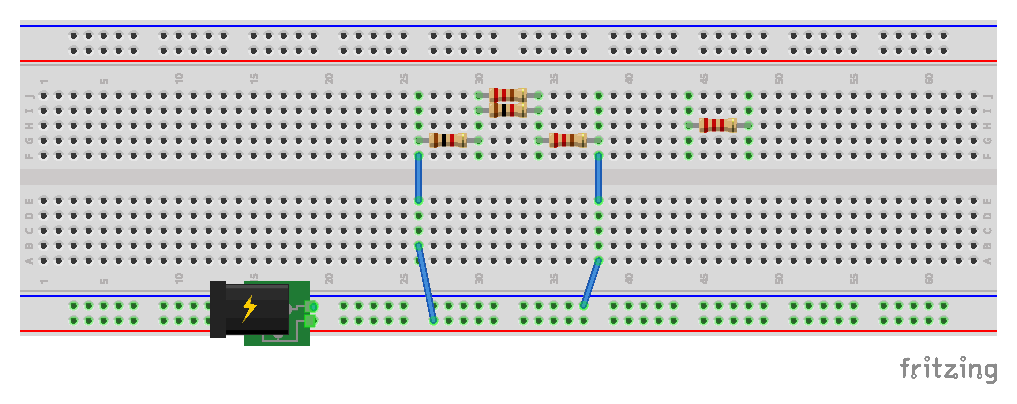
\includegraphics[scale=0.8]{R3_pomiar_napiecia_bb.pdf}
			\captionof{figure}{Schemat badanego obwodu przygotowanego do pomiaru napięcia.}
		\end{figure}
		
		Zastąpienie źródła napięcia i pomiar rezystancji zastępczej $R_{th}$ przy użyciu multimetru skonfigurowanego do pomiaru rezystancji. Multimetr wskazał wynik: $ 154,512\Omega $.
		\begin{figure}[H]
			\centering
			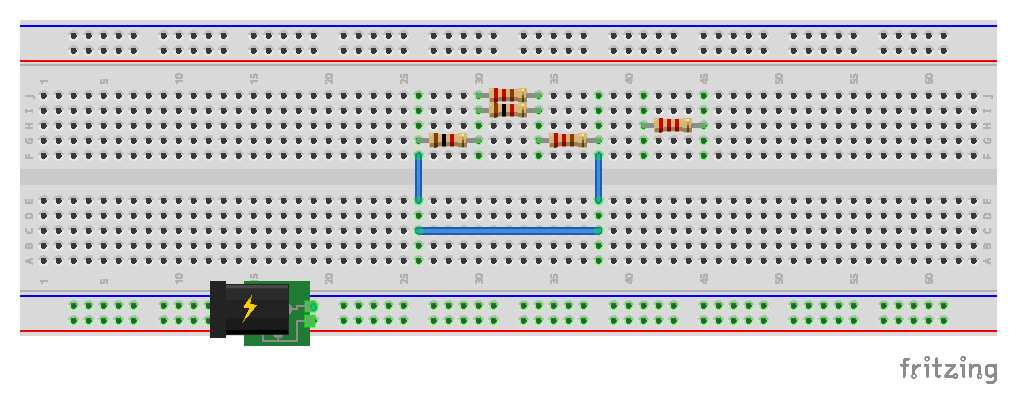
\includegraphics[scale=0.8]{R3_pomiar_oporu_bb.pdf}
			\captionof{figure}{Schemat badanego obwodu przygotowanego do pomiaru rezystancji zastępczej.}
		\end{figure}
		Wyznaczenie prądu $I_{3}$, z wartości otrzymanych podczas pomiarów, przy pomocy wzoru: $I_{x}= \dfrac{U_{thx}}{R_{thx} + R_{x}}$.
		\begin{gather*}
		I_{3}=\dfrac{0.658V}{154.512\Omega + 2200\Omega } = 0.279mA
		\end{gather*}
	\subsubsection{Przy pomocy obliczeń analitycznych}
	Obliczenie $U_{ht}$ przy wyeliminowanym oporniku $ R_{3} $.
			\begin{gather*}
	U_{th}= \dfrac{V_{1}}{R_{4}+R_{5}+R_{12}} \cdot R_{12}\\
	R_{12} = \dfrac{R_{1} \cdot R_{2}}{R_{1} + R_{2}}\\
	R_{12} = \dfrac{220000\Omega}{1220\Omega} = 180.33\Omega\\
	U_{th} = \dfrac{5V}{1000\Omega + 220\Omega + 180.33\Omega } \cot 180.33\Omega\\
	U_{th} = 0.644V
	\end{gather*}
		Obliczenie $R_{ht}$ przy wyeliminowanym oporniku $ R_{3} $.
	\begin{gather*}
	R_{21} = \dfrac{1}{\dfrac{1}{R_{2}} + \dfrac{1}{R_{1}}}\\
	R_{45} = R_{4} + R_{5}\\
	R_{th} = \dfrac{1}{\dfrac{1}{R_{21}} + \dfrac{1}{R_{45}}} = \dfrac{1}{\dfrac{1}{\dfrac{1}{\dfrac{1}{R_{2}} + \dfrac{1}{R_{1}}}} + \dfrac{1}{R_{4} + R_{5}}}\\
	R_{th} = \dfrac{1}{\dfrac{1}{\dfrac{1}{\dfrac{1}{2200\Omega} + \dfrac{1}{220\Omega}}} + \dfrac{1}{1000\Omega + 220\Omega}} \approx 157,106\Omega
	\end{gather*}
		Wyznaczenie prądu $I_{3}$, z wartości otrzymanych podczas obliczeń, przy pomocy wzoru: $I_{x}= \dfrac{U_{thx}}{R_{thx} + R_{x}}$.
	\begin{gather*}
	I_{3}=\dfrac{0.644V}{154,512\Omega + 2200\Omega } = 0.273mA
	\end{gather*}
	\section{Zestawienie wszystkich wyników obliczeń i pomiarów}
		\begin{figure}[H]
			\begin{equation*}
			\begin{array}{|c|c|c|c|c|c|c|}
				\cline{2-7}
				\multicolumn{1}{c}{}&\multicolumn{3}{|c|}{Pomiar}&\multicolumn{3}{|c|}{Obliczenia}\\
				\cline{2-7}
				\multicolumn{1}{c|}{}&R_{1}&R_{2}&R_{3}&R_{1}&R_{2}&R_{3}\\
				\hline
				U_{th}&1.824V&0.749V&0.658V&1.802V&0.704V&0.644V\\
				\hline
				R_{th}&434.202\Omega&168.841\Omega&154.512\Omega&439,712\Omega&171,831\Omega&157,106\Omega\\
				\hline
				I&2.788mA&0.641mA&0.279mA&2.732mA&0.602mA&0.273mA\\
				\hline
				
			\end{array}
			\end{equation*}
		\end{figure}
	\section{Wnioski z przeprowadzonych badań}
	Po przeanalizowaniu wyników obliczeń i pomiarów można wywnioskować, że zostały one poprawnie przeprowadzone. 
	\section{Zastosowania twierdzenia Thevenina}
	Twierdzenia Thevenina można użyć:
	\begin{itemize}
		\item podczas rozwiązywania układów elektrycznych liniowych 
		\item do uproszczenia obwodów w celu ułatwienia rachunków analitycznych
	\end{itemize}

	\begin{thebibliography}{99}
		\bibitem{pa}  S. Bolkowski,  \emph{Teoria obwodów elektrycznych} , ser. Elektrotechnika teoretyczna. Wydawnictwa NaukowoTechniczne,
		1986, 
	\end{thebibliography}
	\newpage
	\tableofcontents
		
	\end{spacing}
\end{document}


